\documentclass[preprint]{sigplanconf}

% The following \documentclass options may be useful:
%
% 10pt          To set in 10-point type instead of 9-point.
% 11pt          To set in 11-point type instead of 9-point.
% authoryear    To obtain author/year citation style instead of numeric.

\usepackage{amsmath}
\usepackage{graphicx}
\usepackage{url}
\usepackage{amssymb}
\usepackage{subfigure}
\usepackage{algorithm} 
\usepackage{algpseudocode}
\usepackage{epsfig}
\usepackage{fancyvrb}
%\usepackage{times}

% make an environment for subfigures with verbatim
\newbox\subfigbox	% Create a box to hold the subfigure. 
\makeatletter
  \newenvironment{subfloat}% % Create the new environment. 
    {\def\caption##1{\gdef\subcapsave{\relax##1}}%
    \let\subcapsave=\@empty % Save the subcaption text.  
    \let\sf@oldlabel=\label 
    \def\label##1{\xdef\sublabsave{\noexpand\label{##1}}}%
    \let\sublabsave\relax  %
    \setbox\subfigbox\hbox 
        \bgroup}% 
     {\egroup   %
    \let\label=\sf@oldlabel
    \subfigure[\subcapsave]{\box\subfigbox}}% 
\makeatother

\newcommand{\eightpoint}{\fontsize{8pt}{10pt}\selectfont}
\newcommand{\ninepoint}{\fontsize{9pt}{11pt}\selectfont}

%\advance \baselineskip by 0.4pt

% do not indent paragraphs of enumerated lists (my lists go on for pages...)
% numbers flush left to paragraph text: \leftmargin=17pt
\newcommand{\mybegin}{\begin{list}{\labelenumi}{\leftmargin=\parindent}\usecounter{enumi}}
\newcommand{\myitem}[1]{\item {\textit{\textbf{#1}}}}
%\newcommand{\myitem}[1]{\item {\bf #1}}
\newcommand{\myend}{\end{list}}
\newcommand{\mt}[1]{\mbox{\it #1}}
\newcommand{\todo}[1]{\framebox {\bf #1}}
\newcommand{\work}{{\tt work()}~}
\newcommand{\prework}{{\tt prework()}~}
\newcommand{\iter}{{\tt iter()}~}


\begin{document}

%\titlebanner{banner above paper title}        % These are ignored unless
%\preprintfooter{short description of paper}   % 'preprint' option specified.

\title{Representing and Parallelizing Induction Variable State in Stream Programs}

\authorinfo{Anonymous}
           {}
           {}

\maketitle

\begin{abstract}
Applications that are structured around some notion of a "stream"
are becoming increasingly important and widespread.  There is
evidence that streaming media applications are already consuming
most of the cycles on consumer machines \cite{Rix98}, and their
use is continuing to grow.  {\StreamIt} is a language and compiler
specifically designed for modern stream programming.  Despite the
prevalence of these applications, there is surprisingly little
language and compiler for practical, large-scale stream
programming.  {\StreamIt} is a language and compiler specifically
designed for modern stream programming.  The {\StreamIt} langauge
holds two goals: first, to provide high-level stream abstractions
that improve programmer productivity and program robustness within
the streaming domain; second, to serve as a common machine
language for grid-based processors.  At the same time, {\StreamIt}
compiler aims to perform stream-specific optimizations to achieve
the performance of an expert programmer.  This thesis develops
several techniques for scheduling execution of {\filters} in
{\StreamIt}.  The work focuses on correctness as well as
minimizing buffering requirements and stored schedule size.

\end{abstract}

%\category{CR-number}{subcategory}{third-level}

%\terms
%term1, term2

%\keywords
%keyword1, keyword2

\section{Introduction}

The domain of stream programs is important because it stands at the
intersection of trends in applications and architectures.  Stream
programming naturally represents applications such as audio, video,
digital signal processing, and data analysis; applications that are
increasing prevalent as computing moves towards data-centric
applications and to the mobile and embedded space.  Also, by virtue of
their structure -- a graph of independent computational nodes (termed
{\it filters}) with explicit and regular communication -- stream
programs are a natural fit for exploiting coarse-grained parallelism
suitable for multicore architectures.  The interest in streaming
applications has spawned a number of streaming languages that target
the streaming domain, including StreamIt~\cite{streamitcc},
Brook~\cite{brook04}, Cg~\cite{cg03},
SPUR~\cite{spur05samos}, Spidle~\cite{spidle03}, Lime~\cite{lime10},
and SPL~\cite{spl09}.

In a stream program, filters define an atomic execution step that
repeats for many iterations; each execution step discards a number of
data items from filter's input edge.  Often, a filter does not discard
all the data items that it read for the current execution step,
requiring these inspected (but not discarded) items for a future
iteration (or iterations) of the filter.  This type of filter is
described as performing a sliding window computation on its
input. Sliding window computations are prevalent in stream programs.
Examples of sliding window computations include FIR filters; moving
averages and differences; error correcting codes; motion estimation;
and network packet inspection.  A recent study of a large streaming
benchmark suite written in the StreamIt programming language finds
that 17 of the 30 real-world benchmarks include at least one filter
that performs a sliding window computation~\cite{streamit-suite}.


Figure~\ref{fig:fir-nopeeking} shows how to perform a sliding
window FIR filter via state carried between iterations of a filter.
This implementation is difficult for the compiler to analyze and
reason about.  Some programming languages (e.g., Brook, Lime,
StreamIt, and IBM SPL) go so far as to include idioms that directly
represent sliding window computation, allowing the programmer to
specify, for each filter, the size of the window and the number of
items discarded after an execution of the filter.
Figure~\ref{fig:fir-peeking} shows how language extensions of the
StreamIt programming language elegantly expose sliding windows for
compiler analysis and optimization.

A goal of stream programming is to directly expose to the software
layer the necessary information to enable automatic management of
coarse-grained parallelism.  Stream programs expose multiple forms of
parallelism: pipeline parallelism that exists between producers and
consumers; task parallelism that exists between pairs of filters on
parallel branches of the stream graph; and data parallelism that
exists when a filter is stateless and can thus be replicated.  Data
parallelism is the most attractive, as it provides load-balanced and
limitless parallelism (as long as input data is available).  A filter
that is stateful, and cannot be data-parallelized, becomes a limit to
parallelization scalability, as the work of that filter cannot be
divided; the most load-intensive stateful filter becomes a
bottleneck.

This paper presents a compiler framework for data-parallelizing
filters that perform sliding window computations when the properties
of the sliding window can be calculated statically.  If sliding window
filters required state, this state would represent a new
parallelization bottleneck.  Sliding windows are the bottleneck in 11
of the 17 real-world benchmarks in the StreamIt Benchmark Suite that
contain sliding windows~\cite{streamit-suite}.  For example, examining
the Channelvocoder benchmark, this state would limit scalability to 18
cores, whereas our techniques scale to at least 64 cores.

Data-parallelizing a filter is performed via a transformation termed
{\it fission} (verb form {\it fiss})~\cite{streamit-asplos}.  Fission
is the process of data-parallelizing a stateless filter by duplicating
the filter a certain number of ways, assigning duplicates to distinct
cores, and correctly distributed input data to and collecting output
data from the duplicates.  The duplicated filters are referred to as
{\it products}.  When a sliding window is present, fission is
accomplished by duplicating certain input items since they are
required by multiple products.  This duplication translates into
inter-core communication, a limiting factor for scalability when
targeting multicore architectures.

Previous approaches duplicate each input data item to all products,
with products ignoring (decimating) items that are not
needed~\cite{streamit-asplos}.  We will show that this strategy limits
scalability for multicores by requiring too much inter-core
communication.  In contrast, our strategy precisely routes each input
item to the minimal set of product filters that requires the item.
Unlike previous work, our techniques are defined on
multiple input and multiple output filters, removing the need to
introduce synchronization filters that serialize data before and
after the product filters.  

Our techniques operate on {\it static-rate} stream graphs, meaning
that the number of items produced, the number of items consumed, and
the number of items inspected by each filter can be determined
statically.  Because of this property, a steady-state schedule of
filter firings can be calculated that does not grow buffers and can be
executed indefinitely~\cite{lee87}.  Our techniques are conscious of
the spatial locality between producers and consumers.  Our framework
includes techniques that can determine when spatial locality can be
increased by altering the steady-state schedule.  When applicable, our
techniques can reduce the overall sharing (and thus inter-core
communication) requirement to below a threshold percent of the total
input communication for each sliding window filter that is
data-parallelized. 

\begin{figure}[t]
\centering
\subfigure[]{\includegraphics[width=3.3in]{figures/fir-nopeeking.pdf}\label{fig:fir-nopeeking}}
\subfigure[]{\includegraphics[width=3.3in]{figures/fir-peeking.pdf}\label{fig:fir-peeking}}
\caption[Two implementations of an FIR filter.]{\label{fig:fir-code}
  Two StreamIt implementations of an FIR filter:
   (a) the non-peeking version implemented via a
  stateful circular buffer; and (b) the peeking version. Only steady-state implementation is
  given.}
\end{figure}

The framework presented is defined on a model of computation that is
agnostic of source language.  To evaluate our techniques we have
implemented them in the context of the StreamIt compiler
infrastructure~\cite{gordon-asplos06}.  Our transformations are guided
by the parallelization management techniques presented
in~\cite{gordon-asplos06}.  We employ 3 real-world benchmarks from the
StreamIt Benchmark Suite~\cite{streamit-suite} that include sliding
window computation.  We demonstrate the effectiveness of our
techniques by comparing them to previously published techniques on 2
multicore architectures: a 16-core SMP shared-memory multicore and the
64-core distributed-memory Tilera TILE64.  We show that
our techniques are required to achieve scalable parallelization on
both architectures, achieving a 6.7x mean speedup on the 16-core SMP
and a 1.8x mean speedup on the 64-core distributed memory multicore
over a previously published technique.

\subsection{Contributions}
This paper makes the following contributions:
\begin{itemize}
  % \myitem{Motivation for Exposing Sliding Windows in Stream
  %   Languages}: Without exposing sliding windows in the language, it
  % requires heroic effort by the compiler to analyze the access patterns
  % of such a filter. Without success, the compiler will not be able to
  % data-parallelize these filters.  This will prevent robust 
  % parallelization scalability for streaming applications.

  \myitem{Generalized Fission of Sliding Window Filters}: We present a
  transformation that fisses sliding window filters with multiple
  input and multiple outputs.  The technique also supports filters
  that with multiple schedules of execution.  General fission defines
  a precise pattern of communication of input data to the products
  that can be reasoned upon by our other techniques.

  \myitem{Sharing Reduction}: We are the first to present a technique
  that decides when it is possible to decrease the amount of sharing
  between fission products by altering the steady-state of a stream
  graph, thus decreasing inter-core communication.  The technique
  reasons about all the sliding window filters of the stream graph,
  and when possible, reduces the sharing requirement to below a given
  threshold percent of the total input of the filters. 

  \myitem{Data Parallelization of Stream Graph}: We present a
  framework for data-parallelizing all of the filters of a stream
  graph employing the fission transformation on individual filters and
  applying sharing reduction when possible.  This framework optimizes
  for spatial locality and enables the compiler to automatically and
  effectively manage parallelization across varying multicore
  architectures.

  \myitem{Enable Robust Parallelization Scaling for Multicores}: For
  streaming applications with sliding window computation, previously
  published data-parallelization transformations do not scale for our
  target multicores. Our techniques enable robust parallelization
  scalability by reducing inter-core communication.  We achieve a 17x
  mean parallelization speedup for a 16-core SMP and a 62.3x mean
  parallelization speedup for the 64-core TILE64 across our benchmarks.

\end{itemize}

% \begin{figure}[t]
% \centering
% \begin{subfloat}
% \begin{minipage}[b]{0.45\textwidth}
% \eightpoint
% \begin{verbatim}
% float->float filter FIR(int N) {
%   int srcBuffer[N];
%   int srcEnd = 0; 
%   ...
%   work push 1 pop 1 {
%     srcBuffer[srcEnd] = pop();
%     float sum = 0;
%     for (int i=0; i<N; i++) {
%       sum += weights[i] * srcBuffer[(srcEnd + i + 1) % N];
%     }
%     push(sum);
%     srcEnd = (srcEnd + 1) % N;
%   }
% }
% \end{verbatim}
% \vspace{-8pt}
% \end{minipage}%
% \caption{ \label{fig:fir-nopeeking}}
% \end{subfloat}%
% \qquad
% \begin{subfloat}
% \begin{minipage}[b]{0.45\textwidth}
% \eightpoint
% \begin{verbatim}
% float->float filter FIR(int N) {
%   ...
%   work push 1 pop 1 peek N {
%     float sum = 0;
%     for (int i=0; i<N; i++) {
%       sum += weights[i] * peek(i);
%     }
%     push(sum);
%     pop();
%   }
% }
% \end{verbatim}
% \vspace{-18pt}
% \end{minipage}
% \caption{ \label{fig:fir-streamit}}
% \end{subfloat}
% \caption[Two implementations of an FIR filter.]{\label{fig:fir-code}
%   Two StreamIt implementations of an FIR filter:
%    \subref{fig:fir-nopeeking} the non-peeking version implemented via a
%   stateful circular buffer; and \subref{fig:fir-streamit} the peeking version. Only steady-state implementation is
%   given.}
% \end{figure}

\section{{\StreamIt} Language}
\label{chpt:streamit}

This chapter introduces relevant constructs of the {\StreamIt}
language.  Syntax is not explored here, as it is not relevant to
{\StreamIt} scheduling.

Section \ref{sec:streamit:struct} introduces the structured
streaming concept, while Section \ref{sec:streamit:messages}
introduces the low bandwidth messaging semantics of {\StreamIt}.

\subsection{Structure}
\label{sec:streamit:struct}

Perhaps the most distinguishing feature of {\StreamIt} language is
that it introduces structure to the concept of stream computation.
{\StreamIt} concept of structure is conceptually similar to
structured constructs in functional languages such as \C.

In {\StreamIt} programs are composed out of streaming components
called streams.  Each stream is a single-input, single-output
component, possibly made up of a hierarchical composition of other
streams. Streams can only be arranged in a limited number of ways,
using {\pipelines}, {\splitjoins}, and {\feedbackloops}.  Data
passed between {\filters} is read from and written to {{\Channels}}.
Figure \ref{fig:structure} contains examples of various
{\StreamIt} streams.  The restrictions on arrangement of streams
enforces the structure imposed by {\StreamIt}.

\begin{figure}\begin{center}
\begin{minipage}{2in}
\centering
\psfig{figure=filter.eps,width=0.7in} \\
{\protect\small (a) A {\filter}}
\end{minipage}
~
\begin{minipage}{2in}
\centering
\psfig{figure=pipeline.eps,width=0.7in} \\
{\protect\small (b) A {\pipeline} with $n$ children.}
\end{minipage}
~
\begin{minipage}{2in}
\centering
\psfig{figure=splitjoin.eps,width=2in} \\
{\protect\small (c) A {\splitjoin} with $n$ children}
\end{minipage}
~
\begin{minipage}{2in}
\centering
\psfig{figure=feedback.eps,width=1.5in} \\
{\protect\small (d) A {\feedbackloop}}
\end{minipage}
\end{center}
\caption{All {\StreamIt} streams}
\label{fig:structure}
\end{figure}

\subsubsection{\filters}

The basic unit of computation in {\StreamIt} is the {\filter}. The
central aspect of a filter is the {\work} function, which
describes the filter's atomic execution step. Within the {\work}
function, the filter can communicate with its neighbors using the
{\Input} and {\Output} channels, which are typed FIFO queues
declared during initialization of a {\filter}.  Figure
\ref{fig:structure}(a) depicts a {\filter}.

{\filters} also have the restriction of requiring a static amount
of data to be consumed and produced for each execution of a
{\work} function.  The amount of data produced by a {\filter} $F$
upon execution of its {\work} function is called a push amount,
denoted $push$. The amount of data consumed from {\Input}
{{\Channel}} by a {\filter} $F$ upon execution of its {\work}
function is called a pop amount, denoted $pop$.  {\filters} may
require that additional data be available in the {\Input}
{{\Channel}} for the {\filter} to examine.  This data can be read by
the {\filter}'s {\work} function, but it will not be consumed, and
will remain in the {{\Channel}} for the next execution of the
{\work} function.  The amount of data necessary on the {\Input}
{{\Channel}} to execute {\filter}'s {\work} function is called peek
amount, denoted $peek$.  Note, that for all {\filters} $peek
>= pop$.  Extra peek amount is the amount of data required on by
the {\filter} that will be read but will not be consumed, namely
$peek - pop$.  The \emph{peek}, \emph{pop} and \emph{push} values
in Figure \ref{fig:structure}(a) correspond to the $peek$, $pop$
and $push$ amounts of the {\filter}'s {\work} function.

A {\filter} can be a source, if it does not consume any data, but
it produced data.  Namely, a {\filter} is a source if it has $peek
= pop = 0$. Likewise, a {\filter} can be a sink, if it consumes
data, but does not produce any, or $push = 0$.

\subsubsection{\pipelines}

{\pipelines} are used to connect {\StreamIt} structures in a chain
fashion: each child stream's output is the next child stream's
input. {\pipelines} have no {\work} function, as they do not perform
any computation themselves. {\pipelines} are simply containers of
other {\StreamIt} structures.  Figure \ref{fig:structure}(b) depicts
a {\pipeline}.

\subsubsection{\splitjoins}

{\splitjoins} are used to specify independent parallel structures
that diverge from a common {\splitter} and merge into a common
{\joiner}.  There are two types of {\splitters}:
\begin{enumerate}[(a)]
\item %(a)
{\duplicate}, which replicates each data item and sends a copy to
each parallel stream, and

\item %(b)
{\roundrobin} $(w_0,\dots, w_{n-1})$, which sends the first $w_0$
items to the first stream, the next $w_1$ items to the second
stream, and so on.  If all $w_i$ are equal to $0$, all child
streams of the {\splitjoin} must be sources.
\end{enumerate}

{\roundrobin} is also the only type of a {\joiner} supported in
{\StreamIt}; its function is analogous to a {\roundrobin} {\splitter}.

Figure \ref{fig:structure}(c) depicts a
{\splitjoin}.

\subsubsection{\feedbackloops}
\label{sec:explain-fl}

{\feedbackloops} are used to create cycles in the stream graph. A
{\feedbackloop} contains a {\joiner}, a body stream, a {\splitter}, and
a loop stream.  Figure \ref{fig:structure}(d) depicts a
{\feedbackloop}.

A {\feedbackloop} has an additional feature required to allow a
{\feedbackloop} to begin computation: since there is no data on
the feedback path at first, the stream instead inputs data from a
special function defined by the {\feedbackloop}.  The amount of
data pushed onto the feedback path is called delay amount, denoted
$delay_{fl}$, for a {\feedbackloop} $fl$.

\subsection{Messages}
\label{sec:streamit:messages}

In addition to passing data between {\filters} using structured
streams, {\StreamIt} provides a method for low-bandwidth data
passing, similar to a combination of sending messages and function
calls. Messages are sent from within the body of a {\filter}'s
{\work} function, perhaps to change a parameter in another
{\filter}. The sender can continue to execute while the message is
en route. When the message arrives at its destination, a special
message receiver method is called within the destination
{\filter}. Since message delivery is asynchronous, there can be no
return value; only void methods can be message targets. This
allows the send to continue execution while the message is en
route - the sender does not have to wait for the receiver to
receive the message and send a return value back. If the receiver
wants to send a return value to the sender, it can send a message
back to the sender.

Although message delivery in {\StreamIt} is asynchronous in
principle, {\StreamIt} does include semantics to restrict the
latency of delivery of a message. Since {\StreamIt} does not
provide any shared resources to {\filters} (including global
memory, global clock, etc), the timing mechanism uses a concept of
flow of information.

One motivating example for messaging in {\StreamIt} can be found in
cell phone processing application. Modern cellular phone protocols
involve a technique called frequency hopping - the cell phone base
station selects a new frequency or channel for the phone to
communicate with the base station and informs the phone of this
change.  The phone must switch to the new channel within a certain
amount of time, or it risks losing connection with the base
station.

If the phone decoder application is written in {\StreamIt}, the
{\filter} controlling the antenna and the {\filter} which will process
control signals are likely far apart, and may not have a simple
way of communicating data directly with each other. In {\StreamIt},
the {\filter} which decodes control signals can simply send a
message to the {\filter} controlling the antenna. The message can be
sent with a specific latency corresponding to the timing required
by the base station. When the antenna controller receives the
message it can change the appropriate settings in the hardware to
switch to the appropriate new frequency, without having to wait
for the appropriate time. The timing of delivery is taken care of
by {\StreamIt}.

\subsubsection{Information Wavefronts}

When a data item enters a stream, it carries with it some new
information. As execution progresses, this information cascades
through the stream, affecting the state of {\filters} and the values
of new data items which are produced. We refer to an information
wavefront as the set of {\filter} executions that first sees the
effects of a given input item. Thus, although each {\filter}'s {\work}
function is invoked asynchronously without any notion of global
time, two invocations of a work function occur at the same
information-relative time if they operate on the same information
wavefront.

\subsubsection{Message Sending}

Messages can be sent upstream or downstream between any two
{\filters}.  Sending messages across branches of a {\splitjoin} is not
legal.  Timing of message delivery uses the concept of information
wavefront.  The sender specifies that the message is supposed to
be delivered with a certain delay of information wavefront. The
delays are specified as ranges, $[l_0, l_1], l_0 \le l_1$. $l_0$
and $l_1$ specify the information wavefront in executions of the
{\work} function of the sender {\filter}.

If the message is being sent downstream, the sender specifies that
the receiver will receive the data just before it sees the
information wavefront produced by the sender between $l_0$ and
$l_1$ executions of its {\work} function from when it sends the
message. If the message is being sent upstream, the sender
specifies that the receiver must receive the message just before
it produces an information wavefront the sender will see between
$l_0$ and $l_1$ executions of its {\work} function from when it
sends the message.

Message sending is meant to be a low-bandwidth method of
communication between {\filters}. Message sending is not a fast
operation and is intended not to interfere with the high bandwidth
{\StreamIt} communication and processing.  However, depending on how
tight the latency constraints are (both the magnitude of the
latency as well as the range), declaring that messages can be sent
may slow program execution down considerably.

Figure \ref{fig:message-example} presents an example of a
{\pipeline} in which the last {\filter} sends a message to the first
{\filter}.  {\filter}$_3$ sends a message to {\filter}$_0$.  The message
is sent with latency $[3,8]$. This means that after at least 3 and
at most 8 executions of sender's {\work} function, it will see data
produced by the receiver just after receiving the message.

\begin{figure}\begin{center}
\begin{minipage}{4in}
\centering
\psfig{figure=message-example.eps,width=1.5in} \\
\end{minipage}
\end{center}
\caption{Example of a {\pipeline} with a message being sent}
\label{fig:message-example}
\end{figure}

\section{Induction Variable State in Stream Programs}
\label{sec:inductionstate}

% \begin{figure}[t]
% {\eightpoint
% \begin{verbatim}
%   int->int stateful filter InductionFilter() {
%       int counter;
%       int max;
  
%       work push 1 pop 1{

%           ...

%           counter = (counter + 1);

%           if (counter > max) {
%               counter = 0;
%           } 
%       }
%   }
% \end{verbatim}
% \caption{Example of a stateful StreamIt filter using induction variable state.\protect\label{fig:filter-example}}}
% \end{figure}

Traditional induction variables encapsulate all variables that are
increased or decreased with iterations of a loop.  Induction variable
state as applied to stream programming is a class of state that
requires keeping count of how often a filter has been invoked.  Common
usage of induction variable state include performing some special
action after a certain number of iterations and keeping track of array
index positions.  Many filters maintain multiple induction variables
as well, which may be either dependent or independent of each other.

Many applications in the StreamIt benchmark suite, including MPEG2 encoder,
Medium Pulse Doppler, Trellis, and FIRBank (pipelined version), maintain induction variable state 
by creating a mutable state field in the corresponding filter.  This
state can be set to the desired starting value.  The induction
variable is consistently updated at some point during the work call.
For many use cases, this induction variable may need to be reset if it
reaches a certain threshold. 

Figure~\ref{fig:apt-pipeline} illustrates a common pattern of explicit
induction variable state.  The implementation of the filter maintains
a filter variable {\tt frameno} that is incremented on each call of
the {\tt AssignPictureType}'s work function.  This variable
represents state.  The {\tt framecount} variable is derived
from this state and used in control flow.

As presently constructed, induction variable state for\-ces the
corresponding filter to be run in sequential order.  In providing a
mutable state whose value is dependent on the previous execution step,
it is necessary to run a filter execution step and establish the
induction variable value before moving on to the next execution step.
The tradition fission transformation would not be able to parallelize
this filter without understanding how to properly distribute the
calculation of the state.  As we mention in the introduction, this
could be accomplished using an automatic induction variable
recognizer, but its idiomatic nature may miss many opportunities for
parallelization.  

\subsection{Potential Data Parallelism in Eliminating State}
Table~\ref{fig:benchmarks} indicates programs in the StreamIt benchmark suite that use induction variable filters (not including source filters) in the manner described above.  The StreamIt compiler provides static estimations of work performed in filters.  The above table indicates the work performed in specifically the induction variable filters.

The majority of programs do not have substantial work performed in filters using induction variables; FIRBankPipeline and MPD contain only a few stateful filters whose total work concentration is fairly low.  The MPEG-2 motion estimation subset is the only exception because its stream graph is comprised mostly with stateful filters.  However, eliminating any form of state will have a large impact on runtime performance even on programs with low work concentration in stateful filters.  We model the potential speedups of a particular stateful program in this subsection.  For the purpose of this analysis, we will assume no communication cost between filters.  We will also assume the compiler exposes no pipeline parallelism.  This assumption forces the serialization of stateful filters on the stream graph.

\begin{table}[t]
\includegraphics[width=3.3in]{figures/induction-benchmarks.pdf}
\caption{Benchmarks using induction variable state and estimations on work performed in filters with induction state.\protect\label{fig:benchmarks}}
\end{table}

Let $N$ be the number of cores we are planning to parallelize over.  Let $\sigma$ be the percentage of work performed in stateful filters that can have its state eliminated, in this case solely filters that use induction variable state.  

If $\sigma = 0$, the entire program is stateless.  The program can be fused to coarsen the granularity, then fissed and mapped to all of the available cores.  Each core would perform $\frac{1}{N}$ of the total work.  Thus with no state, the program can exhibit speedups of up to $N$ times the single-core runtime.

For filters that contain stateful work, $1-\sigma$ of the work in the program is considered stateless, and thus can be fissed and assigned to $N$ individual cores.  The stateful filters cannot be parallelized, and is sequential to all work in the program.  The total serialized work is $\frac{1-\sigma}{N} + \sigma$.  Thus the total speedup is the serial work divided by the new parallelized work.  
\begin{eqnarray*}
\dfrac{1}{\frac{1-\sigma}{N} + \sigma} &=& \dfrac{N}{1 + \sigma(N-1)}
\end{eqnarray*}

We can characterize the amount of speedup between a completely stateless program to an equivalent stateful program with $\sigma$ percentage of stateful work.  This is simply:
\begin{eqnarray*}
\dfrac{N}{\frac{N}{1 + \sigma(N-1)}} &=& 1 + \sigma(N-1)
\end{eqnarray*}

\begin{figure}[t!]
\includegraphics[width=3.3in]{figures/theoretic-speedup.pdf}
\caption{Theoretical speedups of stateless programs over corresponding stateful programs with $\sigma$\% stateful work.  \protect\label{fig:theo-speedups}}
\end{figure}

Figure~\ref{fig:theo-speedups} indicates the potential speedups over stateful programs given stateful work percentages and a varying number of cores.  Even benchmarks in the suite that exhibit only 3\% work in stateful filters can exhibit 8x speedups with 256 cores.  Providing a means to remove state from filters that exhibit very small amounts of work relative to the rest of the program can still generate substantial speedups in the near future.


%\begin{figure}[t]
%{\eightpoint
%\begin{verbatim}
%  int->int stateful filter SingleInductionFilter() {
%      int counter;
%      int max;
%  
%      work push 1 pop 1{
%
%          ...
%
%          counter = (counter + C);
%
%          if (counter > max) {
%              counter = 0;
%          } 
%      }
%  }
%\end{verbatim}
%\caption{Stateful StreamIt filter using induction variable state.\protect\label{fig:transform-before-simple}}}
%\end{figure}
%
%\begin{figure}[t]
%{\eightpoint
%\begin{verbatim}
%  int->int filter SingleInductionFilter() {
%      int max;
%  
%      work push 1 pop 1{
%          int counter = (iter() * C) % max;
%
%          ...
%
%      }
%  }
%\end{verbatim}
%\caption{Stateless StreamIt filter using iteration keyword.\protect\label{fig:transform-after-simple}}}
%\end{figure}
%
%
%\begin{figure}[t]
%{\eightpoint
%\begin{verbatim}
%  int->int stateful filter StartingValueInductionFilter() {
%      int counter;
%      int start;
%      int max;
%
%      init {
%          counter = start;
%      }
%  
%      work push 1 pop 1{
%
%          ...
%
%          counter = (counter + 1);
%
%          if (counter > max) {
%              counter = start;
%          } 
%      }
%  }
%\end{verbatim}
%\caption{Stateful StreamIt filter using induction variable state starting at and resetting to a special starting value.\protect\label{fig:transform-before-starting}}}
%\end{figure}
%
%\begin{figure}[t]
%{\eightpoint
%\begin{verbatim}
%  int->int filter StartingValueInductionFilter() {
%      int max;
%      int start;
%  
%      work push 1 pop 1{
%          int counter = iter() % (max - start) + start;
%
%          ...
%
%      }
%  }
%\end{verbatim}
%\caption{Stateless StreamIt filter using iteration keyword starting at and resetting to a special starting value.\protect\label{fig:transform-after-starting}}}
%\end{figure}
%
%\begin{figure}[t]
%{\eightpoint
%\begin{verbatim}
%  int->int stateful filter TwoNestedInductionFilter() {
%      int counter_x;
%      int counter_y;
%      int max_x;
%      int max_y;
%  
%      work push 1 pop 1{
%
%          ...
%
%          counter_x = (counter_x + 1);
%
%          if (counter_x > max_x) {
%              counter_x = 0;
%              counter_y = (counter_y + 1);
%
%              if (counter_y > max_y) {
%                  counter_y = 0
%              }
%          } 
%      }
%  }
%\end{verbatim}
%\caption{Stateful StreamIt filter using induction variable state starting at and resetting to a special starting value.\protect\label{fig:transform-before-twonested}}}
%\end{figure}
%
%\begin{figure}[t]
%{\eightpoint
%\begin{verbatim}
%  int->int filter TwoNestedInductionFilter() {
%      int max_x;
%      int max_y;
%    
%      work push 1 pop 1{
%          int counter_x = (iter() % max_x);
%          int counter_y = (iter() / max_x) % max_y;
%
%          ...
%
%      }
%  }
%\end{verbatim}
%\caption{Stateless StreamIt filter using iteration keyword starting at and resetting to a special starting value.\protect\label{fig:transform-after-twonested}}}
%\end{figure}


\begin{figure}[t]
\includegraphics[width=3.5in]{figures/transformation1.pdf}
\caption{Translation of a simple filter with induction variable state that resets after a certain value. \protect\label{fig:transform-after-simple}}
\end{figure}

\begin{figure}[t]
\includegraphics[width=3.5in]{figures/transformation2.pdf}
\caption{Translation of a simple filter with induction variable state that resets to a special value. \protect\label{fig:transform-after-start}}
\end{figure}

\begin{figure}[t]
\includegraphics[width=3.5in]{figures/transformation3.pdf}
\caption{Translation of a filter with nested induction variables. \protect\label{fig:transform-after-twonested}}
\end{figure}

Programmers should not have to worry about how to introduce data parallelism into their programs.  With the introduction of a new language construct, hereafter referred to as {\tt iter()}, the programmer can take measures to write their programs to expose data parallelism.  Use of {\tt iter()} potentially provides further benefits in programmability and code readability as well.

The transformation from filters using induction variable state to using {\tt iter()} is fairly simple for users to implement.  Many of these transformations follow the same approach as induction variable elimination.  User defined induction variables can all be derived from the number of times the filter has been invoked.  Accordingly, the induction variable can be expressed as an arithmetic manipulation of {\tt iter()}.  

As described before, induction variable state requires the user to maintain mutable state, updating such state within the filter invocation, and potentially resetting them when required. The programmer can eliminate much of this code simply by arithmetically manipulating {\tt iter()} usage.  As an example, consider the stateful filter with induction state as defined in ~\ref{fig:transform-after-simple}.  The code necessary for maintaining the {\tt counter} field can all be eliminated using general induction variable elimination techniques.  

For filters that define multiple induction variables, it is possible to redefine these values in terms of {\tt iter()} as well.  It is not necessary to maintain multiple separate values for state.  Independent and nested induction variable state alike can be defined with use of {\tt iter()}.

This approach of using {\tt iter} to define induction variable state helps users write filters in a stateless manner.  The user can think about programming their filters in a stateless manner, and thereby exposing data parallelism. 



\section{Design Rationale}

Our approach in removing induction variable state is to introduce a new language construct.  The language construct maintains a value indicating how often the corresponding filter has been invoked.  This approach was chosen over implementing a system to automatically recognize induction variable usage in filter construction.

The approach of automatic analysis would require looking for an induction variable defined in the filter.  The simplest form of this analysis would require first idiomatically detecting for a variable modified by a statement similar to \texttt{var = var + 1}.  Very few iteration filters (outside of source filters) use induction state in this limited capacity.  Consider Figure~\ref{fig:weight-calc}, where the induction variable is incremented at each iteration step, until a certain threshold value at which it will reset.  This pattern is very common in programs that use induction filters.  MPD and FIRBank use this technique to iterate across a provided array one element per iteration step.  To ensure consistency between iteration steps, the automatic analysis is required to detect these types of updates as well.  

\begin{figure}[t]
{\eightpoint
\begin{verbatim}
float->float stateful filter WeightCalc(int n)
{
  float[n] window;
  int windowPos;

  ...

  // the input stream is multiplied with the weights
  work push 2 pop 2
  {

    push(pop() * window[windowPos]);
    push(pop() * window[windowPos]);

    windowPos++;
    if(windowPos >= n)
    {
      windowPos = 0;
    }
  }
}
\end{verbatim}
\caption{MPD filter that multiplies stream values with weights.\protect\label{fig:weight-calc}}}
\end{figure}

\begin{figure}[t]
{\eightpoint
\begin{verbatim}
float->float stateful filter CFARDetectFilter(int rows, int cols)
{
  int currentCol;
  int currentRow;

    ...

  work pop 3 push 1
  {
      ...

    currentRow++;
    if(currentRow >= rows)
    {
      currentRow = 0;

      currentCol++;
      if(currentCol >= cols)
      {
        currentCol = 0;
      }
    }
  }
}
\end{verbatim}
\caption{MPD CFAR Detect filter.\protect\label{fig:cfar-detect-filter}}}
\end{figure}

A filter may have multiple induction variables that are dependent on one another in defining their values.  Consider Figure~\ref{fig:cfar-detect-filter}, a filter used in MPD maintaining nested induction variables.  The automatic analysis must also be able to detect incrementing statements that may not necessarily be updated on every work call.  The process of simply detecting and identifying induction variables can potentially branch into many cases that need to be specially implemented.

There may potentially be other special cases that must be defined into the automatic analysis.  Filters may have also define induction variables to start with and reset to a particular value.  Induction variables may increment by a different value other than 1 at each execution step.  Though the methods of using induction variables as illustrated in Figure~\ref{fig:cfar-detect-filter} and Figure~\ref{fig:weight-calc} encompass many of the common use cases in the benchmark suite, slight variations in the implementation to the pattern may prevent the induction variable from being detected.

Accordingly, there are several downsides to the approach of automatic analysis.  Automatic recognition is a fairly inflexible process in detecting induction variable state.  As illustrated, there may be many different ways of defining induction variables.  Nested counters are often used to track row and column indexes in two-dimensional arrays.  Co-induction variables may be constructed to reset the value of other variables after reaching a certain value.  The many different uses of induction variables may be difficult to assess.  Automatic recognition would restrict data parallelism opportunities to only the filters that fit the implemented templates.  We instead elect to provide the user with the flexibility of defining derived induction values while providing parallelism opportunities.  

The keyword solution also has the added benefit of maintaining a value that is predictable in its updates.  The value that the keyword returns is simply the current iteration number for that the corresponding filter has run.  This is a value that always increments by one at the end of every work call.  Automatic recognition is a frail process because it is difficult to predict how the induction value will be updated, as illustrated in the above figures.  

The approach of automatic analysis also does little to encourage programming with parallelism in mind.  User written code will still maintain state, which inhibits data parallelism opportunities.  In introducing a language construct, user written code eliminates explicitly kept state.  This approach encourages users to write code with the intention of exploiting parallelism.



\subsection{Comparison to Coarsening}
\label{sec:coarsen}

% \begin{figure}[t]
% {\eightpoint
% \begin{verbatim}
% float->float stateful filter WeightCalc(int n)
% {
%   float[n] window;
%   int windowPos;

%   ...

%   // the input stream is multiplied with the weights
%   work push 2 pop 2
%   {

%     push(pop() * window[windowPos]);
%     push(pop() * window[windowPos]);

%     windowPos++;
%     if(windowPos >= n)
%     {
%       windowPos = 0;
%     }
%   }
% }
% \end{verbatim}
% \caption{MPD filter that multiplies stream values with weights.\protect\label{fig:weight-calc}}}
% \end{figure}

In cases of explicit induction variable state where the induction
variable is reset after a certain number of iterations, the filter can
be converted into a stateless filter by {\it coarsening} the filter,
increasing the number of input items that are required for the work
function execution.  Figure~\ref{fig:wc-example}(a) lists the weight
calculation filter from the Medium Pulse Dopler (MPD) benchmark.  The
filter includes explicit induction variable state as originally
implemented by the programmer.  This filter can be rewritten without
state (and without using the {\tt iter()} keyword) by coarsening the
filter such that each work function execution operates on a larger
subset of the input.  Figure~\ref{fig:wc-example}(b) lists a coarsened
implementation that is stateless.  In the coarsened implementation the
filter requires $2n$ input items.

Figure~\ref{fig:wc-example}(c) lists the implementation of the weights
calculation filter utilizing the {\tt iter()} keyword.  Notice that
the filter operates at a finer granularity versus the coarsened
version and that it operates at the same granularity as the original
filter.  Although the {\tt iter()} implementation includes a modulo
operation per output, calculation of outputs will be parallelized
(see Section~\ref{sec:fission}).

The mantra of stream programming is that the programmer should not be
burdened with parallelization, granularity, communication or
synchronization concerns.  Implementing a filter at a fine granularity
allows the compiler or runtime to decide on the best granularity for a
given architectural target.  In practice the use of the {\tt iter()}
keyword is preferred over a coarsening conversion because:

\begin{itemize}

\item The programmer grasped the algorithm and implemented the
  application at the fine granularity.  A language should constrain
  the programmer as little as possible for the sake of performance.

\item The coarse granularity implementation requires larger input and
output buffers to implement because of the larger push and pop rates.
Larger buffers occupy more of the cache and could evict filter data or
instructions are needed during execution.  Thus there could be more
accesses to longer latency memory hierarchies~\cite{sermulins-lctes05}.

\item Larger input and output rates also interact with the
  steady-state scheduling algorithm.  Since the scheduling algorithm
  is performing many cascading LCMs, a single filter with large input
  and output rates will increase the multiplies of all filters of the
  application, requiring more buffering and increasing
  latency~\cite{karczmarek-lctes03}.  The use of the {\tt iter()}
  keyword does not force the programmer to sacrifice latency for
  parallelization.

\end{itemize}


\section{Desugaring}
\label{sec:desugar}

%\begin{figure}[t]
%{\eightpoint
%\begin{verbatim}
%  int->int filter IterationFilter() {
%
%      work push 1 pop 1{
%
%          int counter = iter();
%          ...
%
%      }
%  }
%\end{verbatim}
%\caption{Example of a StreamIt filter using the iteration keyword.\protect\label{fig:iter-filter-example}}}
%\end{figure}
%
%
%\begin{figure}[t]
%{\eightpoint	
%\begin{verbatim}
%  int->int filter IterationFilter() {
%
%      int iter = 0;      
%
%      work push 1 pop 1{
%
%          int counter = iter;
%          ...
%
%          iter++;
%
%      }
%  }
%\end{verbatim}
%\caption{Example of a StreamIt filter with the iteration keyword desugared.\protect\label{fig:desugar-filter-example}}}
%\end{figure}


\begin{figure}[t!]
\centering
\includegraphics[width=3.3in]{figures/desugaring_filters.pdf} 
\caption{Desugaring a filter using \texttt{iter()} keyword.\protect\label{fig:desugar}}
\end{figure}


A filter is classified as an {\it iteration filter} when there exists a use of
\iter in its \prework or \work function.  In this section, we
introduce a simple desugaring transformation that will convert an
iteration filter into a filter that does not include the \iter
keyword, but implements the correct semantics of the \iter use.  We
accomplish this by introducing a state field that records the current
iteration of this filter.  This state field is updated in a consistent
and compiler-defined manner, so later transformations and passes (such
as fission, see \S\ref{sec:fission}) can reason about the
state.  

The \iter expression is replaced with an access to a field holding the
value of the iteration count.  Again, the filter is given a definition
of this field only if it is classified as an iteration filter, this
field is not added to non-iteration filters.  The \work and \prework
function (if it exists) are appended with incrementing statements that
update the iteration value.  The name of the state field is compiler
defined for easy recognition by later passes, for the remainder of
this paper the field is named {\it iter}.


Figure~\ref{fig:desugar} provides a code example of the desugaring
process.  The left filter in Figure~\ref{fig:desugar} shows an
iteration filter.  All references to the keyword are replaced to field
accesses to the {\it iter} field.  Figure~\ref{fig:desugar} shows the
StreamIt code representation after the iteration keyword is desugared.

% The introduction of this iteration field creates state in the provided
% filter.  For future operations, the compiler does not consider this
% iteration field as part of the state of filter.  Future processes will
% maintain this inherent state without the downsides of explicitly
% introduced state.

% It is important to note, these filters are not classified as stateful
% to the user, even though the filter is actually stateful on the
% iteration count after the desugaring process.  In classifying filters
% as stateful, the user is made aware of where data parallelism may be
% inhibited.  Iteration filters will not inhibit data parallelism
% because its state is identifiable to the compiler during the fission
% process.

\subsection{Fission of Induction State}
\label{sec:fission}

\begin{figure}[t!]
\centering
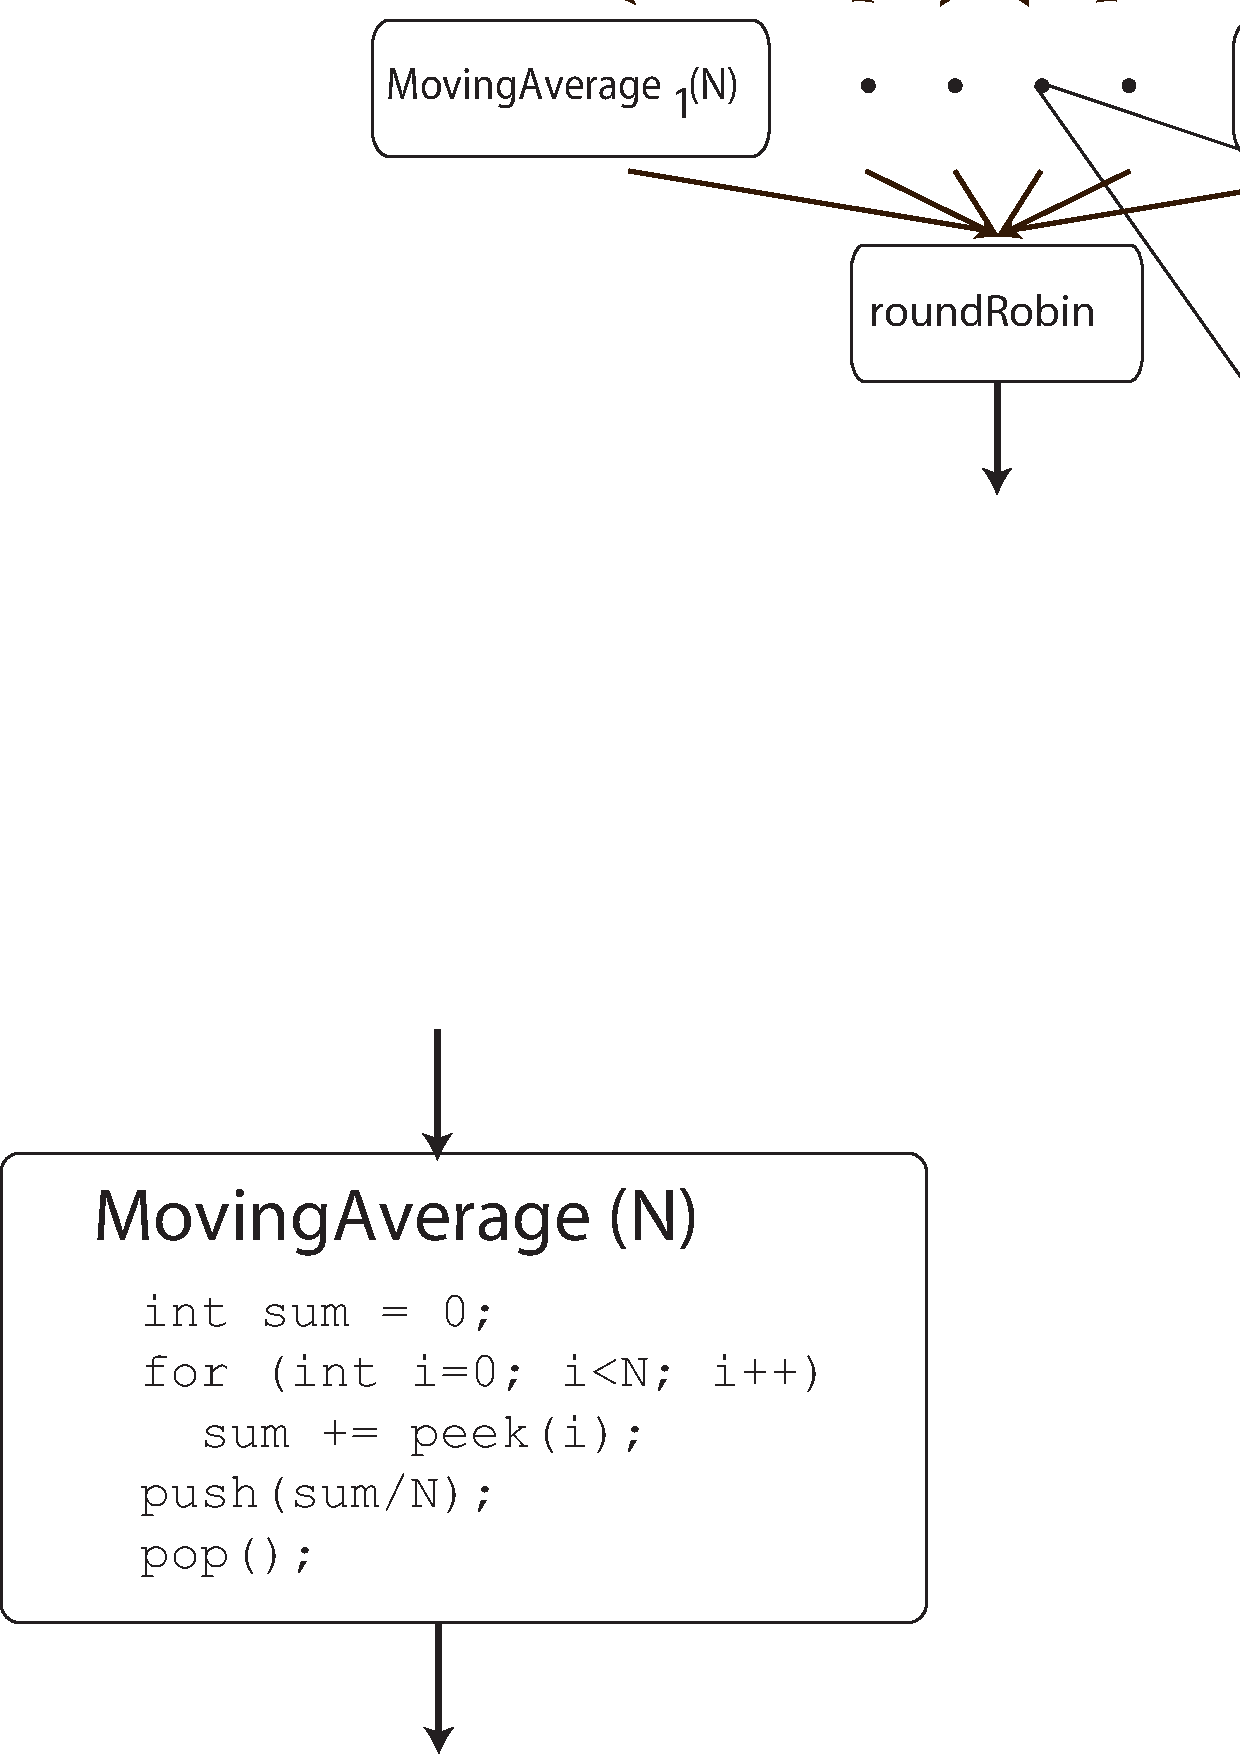
\includegraphics[width=3.4in]{figures/duplicate-fission.pdf}
\caption{Fission of a filter that peeks. \protect\label{fig:duplicate-fission-example}}
\end{figure}


\begin{figure*}[t!]
\centering
\includegraphics[width=6.5in]{figures/fission-example.pdf}
\caption{Example of an iteration filter fissed into three fission products each with multiplicity 2.  The chart indicates the values used to determine the next value of the iteration field.  
\protect\label{fig:fission-example}}
\end{figure*}

The compiler introduces data parallelism to the streaming program through a process known as {\it fission}.  Fission is the process of duplicating the stateless filter and wrapping these duplicates in a round-robin splitter and joiner.  The process ensures that input data is distributed correctly and output data is collected in correct order.  The duplicated filters, known as products, can be assigned to individual cores, thus introducing data parallelism.  

Graphically, fission yields a stream graph result as depicted in Figure~\ref{fig:duplicate-fission-example}.  The base filter, MovingAverage, is duplicated into a duplicate splitjoin and joined in a roundrobin fashion.  Each individual MovingAverage$_j$ product has the work function of the base filter with additional bookkeeping measures to maintain the consistency of the channel inputs and outputs.

Fission is applicable only to stateless filters, as the duplication process does not guarantee consistent behavior if filters contain state that changes between iterations.  Because the desugared iteration filters actually use mutable state to keep track of iteration values, the fission process must be modified to handle iteration values.  

\subsubsection{Modifications to Fission Process}

Let $F$ be the stateless filter that will be fissed.  Assume the fission process yields $N$ fissed products.  Accordingly, this yields the fissed products $F_0$, $F_1$, ... , $F_i$, ... , $F_{N-1}$.  The notation $F_{i}$ represents the $(i+1)$th fissed product of filter $F$.

The fission process now modifies the fission products by adding the
following values as fields to the products:
\begin{itemize}
    \item \texttt{init}: the multiplicity of the initialization schedule.  This value is determined for $F$ and is constant for all fissed products.
    \item $\texttt{reps}_i$: how often the \texttt{work} function of the product $F_i$ is
      invoked between rounds.
    \item $\texttt{start}_i$: the value of the induction variable each product $F_i$ starts with, less the initialization multiplicity.  Alternatively, $\sum_{j=0}^{i-1}{\tt reps}_j$ of all fission products preceding the current product.
    \item \texttt{total}: the periodic multiplicity of $F$.  Alternatively $\sum_{j=0}^{N-1}{\tt reps}_j$. This value is the same for all fissed products.
\end{itemize}
As described in ~\ref{sec:compiler-overview}, initialization execution is required for peeking filters to ensure every firing of the periodic steady-state schedule maintains the same number of leftover items on the channel.  This initialization execution of the original filter is transferred entirely to the first fission product.  However, all fission products must take the multiplicity of the initialization schedule into account in their calculations as the multiplicity is adjusted upwards by this value.

Accordingly, the fission product $F_i$ should start each round with iteration values of
\begin{eqnarray*}
\texttt{total}*\texttt{k} + (\texttt{start}_i + \texttt{init})
\end{eqnarray*}
and range up to the value
\begin{eqnarray*}
\texttt{total}*\texttt{k} + (\texttt{start}_i + \texttt{init}) + \texttt{reps}_i - 1
\end{eqnarray*}
where \texttt{k} is a nonnegative integer indicating how many rounds have
been run in the span of the program.  

At the end of each fission product's \texttt{work}, a check must be made to see if it is necessary to increment the induction variable to the next round of values.  This will prevent certain fissed products from making calls with duplicate iteration values.  This check is done after the field incrementing statement.
\begin{eqnarray*}
(\texttt{iter}_{i,k} - (\texttt{start}_i + \texttt{init}) - \texttt{reps}_i) \% \texttt{total} &==& 0
\end{eqnarray*}
This is consistent with the maximum value per round as
indicated above.  Only when we reach this maximum value does subtracting 
$\texttt{start}_i$, \texttt{init}, and $\texttt{reps}_i$ from $\texttt{iter}_i$ leave a value divisible by
\texttt{total}.

Once the fissed product's iteration value has reached
this value, it must be set to:
\begin{eqnarray*}
\texttt{iter}_{i,k+1} &=& \texttt{iter}_{i,k} + (\texttt{total} - \texttt{reps}_i) \\
&=& \texttt{total}*\texttt{k} + (\texttt{start}_i + \texttt{init}) + \texttt{reps}_i \\
&&  \ \ +\ (\texttt{total} - \texttt{reps}_i) \\
&=& \texttt{total}*(\texttt{k+1}) + (\texttt{start}_i + \texttt{init})
\end{eqnarray*}
which is the starting iteration value of the next round, as defined.

\subsubsection{Accounting for Steady-state Schedule Modification}

Other passes may modify the steady-state schedule after fission, increasing the multiplicity of the fission products.  This scales the $\texttt{reps}_i$ field for all products.  $\texttt{start}_i$ and $\texttt{total}$ are dependent on $\texttt{reps}_i$ and must be scaled accordingly.

Assume a pass increases hte steady-state multiplicity of our filter to $m$.  We expect the fission product $F_i$ to start round $k$ with iteration values of 
\begin{eqnarray*}
(\texttt{total}*\texttt{k}*m) + (\texttt{start}_i*m + \texttt{init})
\end{eqnarray*}
The filter should perform $\texttt{reps}_i$*$m$ iterations, thus should range up to value
\begin{eqnarray*}
(\texttt{total}*\texttt{k}*m) + (\texttt{start}_i*m + \texttt{init}) + (\texttt{reps}_i*m) - 1
\end{eqnarray*}

Between rounds, iteration values must be incremented by the actual total number of repetitions that occur.  All fission products perform a total of $\sum(\texttt{reps}_{i}*m)$ repetitions which is simply \texttt{total}*$m$.  Thus, the updating step will still hold:
\begin{eqnarray*}
\texttt{iter}_{i,k+1} &=& \texttt{iter}_{i,k} + (\texttt{total}*m - \texttt{reps}_i*m) \\
&=& \texttt{total}*\texttt{k}*m + (\texttt{start}_i*m + \texttt{init}) + \texttt{reps}_i*m \\
&&  \ \ +\ (\texttt{total}*m - \texttt{reps}_i*m) \\
&=& \texttt{total}*(\texttt{k+1})*m + (\texttt{start}_i*m + \texttt{init})
\end{eqnarray*}

Figure~\ref{fig:fission-example} shows the filter from Figure~\ref{fig:desugar} fissed into three fission products, each with multiplicity 2.  The accompanying charts for each fissed product are as follows:
\begin{itemize}
\item{\tt iter} indicates the value of the {\tt iter} field at the start of the filter invocation.  
\item{\tt iter++} indicates the value of the {\tt iter} field incremented by 1 (which is the value {\tt iter} takes prior to the check.  
\item{\tt check} indicates the value of $(\texttt{iter}_{i,k} - (\texttt{start}_i + \texttt{init}) - \texttt{reps}_i)$, which must be divisible by {\tt total} in order to advance to the next round.  
\item{\tt next} indicates the value {\tt iter} will take at the next invocation of the fissed product.
\end{itemize}
Note that the value of \texttt{iter} jumps to the next round of values with multiplicity 2, as expected.
\section{The StreamIt Compiler}
\label{sec:compiler}


\begin{table*}[t]
\begin{center}
\scriptsize
\begin{tabular}{|l|l|} \hline
{\bf Phase} & {\bf Function} \\
\hline \hline
KOPI Front-end & Parses syntax into a Java-like abstract syntax tree. \\
\hline
SIR Conversion & Converts the AST to the StreamIt IR (SIR). \\
\hline
Graph Expansion & Expands all parameterized structures in the stream graph. \\
\hline
Scheduling & Calculates initialization and steady-state execution orderings for filter firings. \\
\hline
Partitioning & Performs fission and fusion transformations for load balancing. \\
\hline
Layout & Determines minimum-cost placement of filters on grid of Raw tiles. \\
\hline
Communication Scheduling & Orchestrates fine-grained communication between tiles via simulation of the stream graph. \\
\hline
Code generation & Generates code for the tile and switch processors. \\
\hline
\end{tabular}
\caption{\protect\small Phases of the StreamIt compiler.
\label{tab:phases}}
\end{center}
\end{table*}

The phases of the StreamIt compiler are described in
Table~\ref{tab:phases}.  The details of each stage can be found in
~\cite{streamit-asplos}.  The following subsections provide an
overview on the phases of the StreamIt compiler and the changes made
to the corresponding phases to implement the iteration keyword.

\subsection{StreamIt Compiler Overview}
\label{sec:compiler-overview}

The front end is built on top of KOPI, an open-source compiler 
infrastructure for Java~\cite{kopi}.  We translate the KOPI syntax 
tree into the StreamIt IR (SIR) that encapsulates the hierarchical 
stream graph.  The graph is then expanded for structures that
are parametrized.  Constants are propagated through the program
and the graph is expanded into a static structure.

We can calculate an execution schedule for the nodes of the stream 
graph.  The schedule indicates a multiplicity for each filter in the
stream graph, which determines how often the work function should be
invoked.  The schedule is periodic, meaning its
execution must preserve the number of live items on each channel in
the graph.  Accordingly, there is a {\it steady-state} schedule that is 
periodic which maintains this invariant.  Peeking filters, however, 
introduce another layer of complication.
A filter with {\it peek $>$ pop} leaves {\it peek - pop} items on the
input channel after every firing.  If the periodic schedule contains
these extra items, every firing would leave leftover items
in the channel.  Accordingly, peeking filters require a separate,
non-periodic {\it intialization} schedule.  

{\it Partitioning} is the process of dividing the stream program into
a set of balanced computation units.  Given a number $N$, representing
the maximum number of computation units that can be supported, the 
partitioning step transforms a stream graph into a set of at most $N$
load-balanced filters.  Each filter can be run on a separate processor.
The partitioning step uses a set of fusion, fission, and reordering 
transformations to achieve the desired granularity and load-balancing~\cite{streamit-asplos}.

The {\it layout} phase assigns nodes in the stream graph to the
computation nodes in the target architecture while minimizing the
communication and synchronization in the final layout.  The {\it
communication scheduling} phase maps the communication explicit
in the stream graph to the interconnect of the target.  The FIFO
abstraction of the stream channels is mapped to the limited resources
of the target.  Finally, {\it code generation} is performed using the
results of all previous phases.  
\section{Empirical Evaluation}
\label{sec:analysis}

In this section we evaluate the performance and scalability benefits
of the \iter keyword and its parallelization by providing empirical
results for two applications that originally included induction
variable state. We modified these applications to remove the explicit
induction variable state, and instead employ the \iter keyword. We
modified the StreamIt compiler as described in the last section.  The
experimental architecture is composed of 4 octal-core 2.00 GHz Intel
Xeon x7550 processors, each with 18 MB L3 caches. The architecture has
128 GB of available memory.

\subsection{MPEG-2 Motion Estimation}
\label{sec:mpeg}

\begin{figure}[t]
\includegraphics[width=3.3in]{figures/work_estimate_mpeg_motionestimation.pdf}
\caption{MPEG Motion Estimation stream graph.\protect\label{fig:mpegMEgraph}}
\end{figure}


This section presents an application of induction variables to the Motion Estimation compression subset of the MPEG-2 encoder.  Motion estimation attempts to generate predictions with respect to a set of reference frames obtained from previous or future pictures.  

The stream subgraph of the MPEG-2 encoder is illustrated in Figure~\ref{fig:mpegMEgraph}~\cite{drake-thesis}.  Each block of pixels will be tested against three types of prediction (no prediction, forward predicted, and backward predicted) to determine which is the best method for motion estimation.  The MotionEstimationDecision filter determines which is the best encoding technique for this macroblock.

The filter MotionEstimation is stateful and contains the majority of the work.  The MotionEstimation iterates through a two-dimensional array (16x16 macroblocks) along the picture and relies on induction variables to maintain its array position.  We can apply the induction variable transformation on this filter to remove the state in the filter.

Reference pictures can be set using upstream messaging from later in the stream graph.  Currently the backend does not support the use of upstream messaging, so for the purpose of benchmarking this application, the reference picture is set to a dummy value and is unchanged throughout the program.  This does not detract from the data parallelism introduced after removing the induction state.  Upstream messaging would simply require that sent messages be duplicated to all fissed filters in the stream graph.

\begin{figure}[t]
\includegraphics[width=3.3in]{figures/mpeg-results.pdf}
\caption{Speedups for MPEG-2 Encoder Motion Estimation subset, with and without induction variable state.  \protect\label{fig:mpeg-results}}
\end{figure}

Figure~\ref{fig:mpeg-results} shows the speedup figures for the MPEG-2 motion estimation subset.  There is a noticeable speedup for 2 cores for both induction state and iteration keyword implementations.  This can be attributed to the stream graph, which is composed of two stateful MotionEstimation filters that can be task parallelized.  The bottleneck in data parallelism is apparent as we increase the number of cores past 2, as the majority of the work cannot be partitioned and load-balanced effectively across multiple cores.  

{\it Theoretical speedup} is calculated using the theoretical speedup value from \label{sec:model-analysis} and the base induction state runtime values.  However, this particular stream graph does not allow for all filters to be serialized.  Since the majority of the work is embedded in the two filters that are task parallelizable, we can estimate the theoretical speedups by dividing the theoretical speedup value from \label{sec:model-analysis} by 2.  This is reflected in Figure~\ref{fig:mpeg-results}.

We can see significant improvements to runtime after making this subset stateless and exposing data parallelism.  There is a 4.93X speedup on 8 cores, 9.30X speedup on 16 cores, and 15.62X speedup on 32 cores between the base induction variable and iteration keyword implementations.  

\subsection{FIRBank}
\begin{figure}[t]
\includegraphics[width=3.3in]{figures/firbank-results.pdf}
\caption{Speedups for FIRBank, with and without induction variable state.  \protect\label{fig:firbank-results}}
\end{figure}

The FIRBank benchmark contains multiple finite impulse response
filters each with a different impulse response coefficient array. This
benchmark is used in speech processing applications. FIRBank contains
one filter that uses induction variable state with 3.94\% of program's
work. This filter, Multiply, maintains induction state in an index
that traces through the rows of a two dimensional array. Each
invocation performs complex multiplication on the stream input values
and the array elements of that specified row.  The conversion to the
\iter keyword version removed 5 lines and added 1 line.

The original version with explicit state is partitioned into a 3
filter pipeline: stateless filter, stateful filter (with explicit
induction state), and a stateless filter. The stateless filters are
data-parallelized, but the first requires data to be collected in a
joiner (in a synchronization point) before passing on to the
unparallelized stateful filter. Furthermore, output from the stateful
filter must be communicated to all cores of the chip as the last
stateless filter has fission products on all cores.  In the \iter
version, the entire application is fused to a single filter that can
be data parallelized.  There is no inter-core communication in the
fused and parallelized final version.

Figure~\ref{fig:firbank-results} indicates the speedups over 1 core
for both induction state and iteration keyword implementations.
Between the two implementations, there is 1.36X speedup on 8 cores,
1.58X speedup on 16 cores, and 1.83X speedup on 32 cores for the
iteration keyword implementation. This abides fairly closely with the
model as described in Section ~\ref{sec:model-analysis}.

\section{MPEG-2 Motion Estimation Subset}

This section presents an application of induction variables to the Motion Estimation compression subset of the MPEG-2 encoder.  MPEG-2 is a standard for coding moving pictures and audio information and has a wide variety of multimedia applications.  

The specification contains various types of compression, one of which is motion prediction.  Motion prediction is a lossless compression, or one that eliminates redundant information from a signal while allowing for an exact reconstruction.  Motion prediction takes advantage of the fact that frames of a video contain a large amount of temporal redundancy.  A particular video sequence often contains duplicated scenes between consecutive frames.  Motion estimation attempts to generate motion predictions with respect to a set of reference frames.  These reference frames can be obtained from previous pictures or from both previous and future pictures.  Accordingly, the MPEG-2 encoder can utilize forward and backward motion estimation to achieve this form of compression.

The MPEG-2 standard organizes pictures into 16x16 groups of pixels called macroblocks.  Each macroblock is itself comprised of four 8x8 blocks of pixels termed as blocks.  Macroblocks can be encoded without any motion prediction, known as intra coded pictures, with only forward motion prediction, known as predictive coded pictures, and with both forward and backward motion prediction, known as bidirectionally predictive coded pictures.  These macroblocks are the basis of MPEG-2 motion prediction.  

The process of Motion Estimation entails comparing macroblocks between frames.  The motion estimator forms a motion vector that indicates a cartesian displacement of the macroblock from the most similar macroblock in the reference frames.  The matching macroblock is also removed from the new macroblock, yielding a residual macroblock that contains the difference between the prediction and the actual macroblock being encoded.  

The Motion estimation stream subgraph of the MPEG-2 encoder is illustrated in Figure~ref{}.  Each macroblock will be tested against all three types of prediction (intra coded, forward predicted, and backward predicted) to determine which is the best method for motion estimation.  The MotionEstimationDecision filter determines of these results, which is the best encoding technique.

[cite madrake meng 06]

The work estimation of this compression indicates the filter MotionEstimation is stateful and contains the majority of the work.  The duplicate splitjoin sends a copy of the picture to both forward and backward MotionEstimation and IntraMotionPrediction.  The MotionEstimation filter pulls macroblocks at a time, iterating through a two-dimensional array (16x16 macroblocks) along the picture.  The filter relies on induction variables to maintain its array position.  We can apply the induction variable transformation on this filter to remove this induction state.

Figure~ref{} shows the runtime figures for the original stateful MPEG-2 motion estimation subset compared to the stateless subset.  
\section{Related Work}
\label{sec:related}


The process of eliminating traditional induction variables has been
extensively researched~\cite{Bacon:1994,RM99:RRV}.  These particular
optimizations help eliminate instructions by redefining all induction
variables in terms of a single induction variable.  Many automatically
parallelizing compiler systems, including Rice Fortran D
~\cite{Hiranandani:1992}, SUIF ~\cite{Wilson:1994}, Polaris
~\cite{Blume:1996}, have also done work to automatically eliminate
such traditional induction variables.

Data parallelism is an important class of parallelism that many stream
programming languages attempt to expose.  Other streaming languages
attempt to expose data parallelism that may be inhibited by state in
different ways.  Brook~\cite{brook04} in particular disallows stateful
programs, thus allowing for extensive data parallelism.



These capabilities enable a programmer to write an application and its
filters at a natural granularity that is independent of
parallelization considerations enabling portable, reusable, and
malleable code.  Furthermore, fine-grained implementations of filters
enables the compiler to perform guided filter fusion that balances
data and instruction cache behavior~\cite{sermulins-lctes05}.


Need to address the coarsening issue.  Brook, which disallows state
would force the user to just coarsen the filter.  Why wouldn't someone
just coarsen?  


\section{Conclusion}

This paper shows that the inter-node dependences of a Cyclo-Static
Dataflow Graph can be cleanly represented as a System of Affine
Recurrence Equations.  In combination with Feautrier's array dataflow
analysis~\cite{Feautrier01} for deducing intra-node dependences, this
establishes the SARE as a unified analysis and optimization framework
for high-level DSP programming models.

We believe that the precise affine dependence framework provided by
the SARE representation will enable a powerful suite of node
optimizations in dataflow graphs.  The SARE is a robust and
well-established framework within the systolic and scientific
communities, with methods for graph parameterization, automatic
parallelization, and storage optimization.  We propose optimizations
such as decimation propagation and node fission that are first
applications of these techniques to the signal processing domain.


% \acks
% Acknowledgments, if needed.

% We recommend abbrvnat bibliography style.
\ninepoint
\bibliographystyle{abbrvnat}
\bibliography{references}


\end{document}

